\documentclass[8pt,a4paper,compress]{beamer}

\usepackage{/home/siyer/lib/slides}

\title{Merge Sort}
\date{}

\begin{document}
\begin{frame}
\vfill
\titlepage
\end{frame}

\begin{frame}
\frametitle{Outline}
\tableofcontents
\end{frame}

\section{Merging}
\begin{frame}[fragile]
\begin{itemize}
\item merge sort is based on a simple operation known as merging: combining two ordered arrays to make one larger ordered array

\item to sort an array, divide it into two halves, sort the two halves (recursively), and then merge the results
\begin{center}
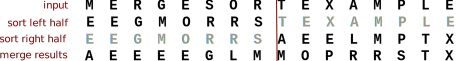
\includegraphics[scale=0.7]{{./figures/mergesort_overview}.pdf}
\end{center}
\end{itemize}
\end{frame}

\begin{frame}[fragile]
\begin{itemize}
\item the merge algorithm
\begin{lstlisting}[language=Java]
    ...
    private static void merge(Comparable[] a, int lo, int mid, int hi) {
        int i = lo, j = mid + 1;
        for (int k = lo; k <= hi; k++) {
            aux[k] = a[k];
        }
        for (int k = lo; k <= hi; k++) {
            if (i > mid) { a[k] = aux[j++]; }
            else if (j > hi ) { a[k] = aux[i++]; }
            else if (less(aux[j], aux[i])) { a[k] = aux[j++]; }
            else { a[k] = aux[i++]; }
        }
    }
    ...
\end{lstlisting}
\end{itemize}
\end{frame}

\begin{frame}[fragile]
\begin{itemize}
\item trace

\begin{center}
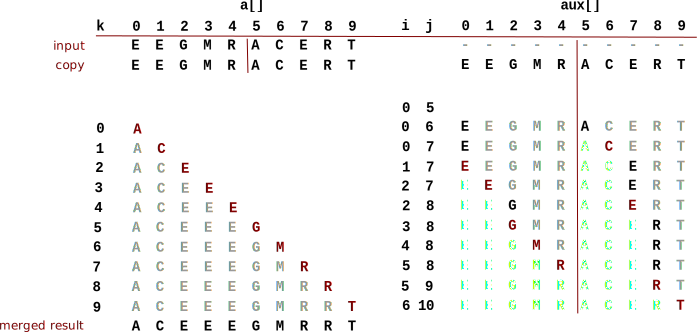
\includegraphics[scale=0.5]{{./figures/merge_trace}.pdf}

\smallskip

the merge algorithm
\end{center}
\end{itemize}
\end{frame}

\section{Merge Sort}
\begin{frame}[fragile]
\begin{itemize}
\item top-down merge sort
\begin{lstlisting}[language=Java]
public class Merge {
    ...
    public static void sort(Comparable[] a) {
        Comparable[] aux = new Comparable[a.length]; 
        sort(a, 0, a.length - 1);
    }
    
    private static void sort(Comparable[] a, int lo, int hi) {
        if (hi <= lo) { return; }
        int mid = lo + (hi - lo) / 2;
        sort(a, lo, mid); 
        sort(a, mid + 1, hi); 
        merge(a, lo, mid, hi);
    }
    ...
}
\end{lstlisting}
\end{itemize}
\end{frame}

\begin{frame}[fragile]
\begin{itemize}
\item trace
\begin{center}
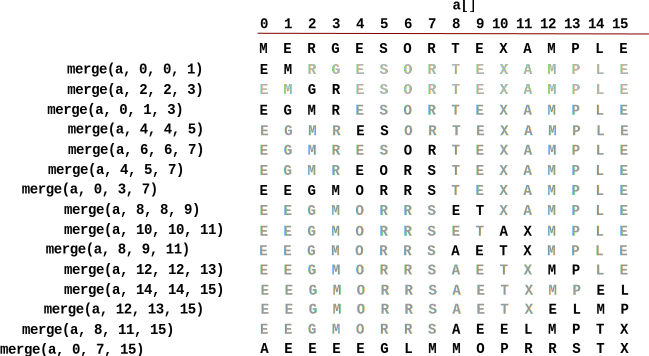
\includegraphics[scale=0.5]{{./figures/mergetd_trace}.pdf}

\smallskip

top-down merge sort
\end{center}
\end{itemize}
\end{frame}

\begin{frame}[fragile]
\begin{itemize}
\item top-down merge sort uses between $1/2N\lg N$ and $N\lg N$ comparisons and at most $6N\lg N$ array accesses to sort an array of length $N$

\item \lstinline$MergeX$ from the text implements the following improvements:

\begin{itemize}
\item tiny subarrays are handled using insertion sort

\item reduces the running time to be linear for arrays that are already in order by adding a test to skip the call to \lstinline$merge()$ if \lstinline$a[mid]$ is less than or equal to \lstinline$a[mid + 1]$

\item eliminates the time (but not the space) taken to copy to the auxiliary array used for merging by using two invocations of the sort method: one that takes its input from the given array and puts the sorted output in the auxiliary array; the other that takes its input from the auxiliary array and puts the sorted output in the given array
\end{itemize}
\end{itemize}
\end{frame}

\begin{frame}[fragile]
\begin{itemize}
\item bottom-up merge sort
\begin{lstlisting}[language=Java]
public class MergeBU {
    ... 
    public static void sort(Comparable[] a) {
        int N = a.length;
        Comparable[] aux = new Comparable[N];
        for (int n = 1; n < N; n = n + n) {
            for (int i = 0; i < N - n; i += n + n) {
                int lo = i;
                int m  = i + n - 1;
                int hi = Math.min(i + n + n - 1, N - 1);
                merge(a, aux, lo, m, hi);
            }
        }
    }
    ...
}
\end{lstlisting}
\end{itemize}
\end{frame}

\begin{frame}[fragile]
\begin{itemize}
\item trace
\begin{center}
\includegraphics[scale=0.5]{{./figures/mergebu_trace}.pdf}

\smallskip 

bottom-up merge sort
\end{center}

\item bottom-up merge sort uses between $1/2N\lg N$ and $N\lg N$ comparisons and at most $6N\lg N$ array accesses to sort an array of length $N$
\end{itemize}
\end{frame}

\section{Complexity of Sorting}
\begin{frame}[fragile]
\begin{itemize}
\item no comparison-based sorting algorithm can guarantee to sort $N$ items with fewer than $\lg N! \sim N\lg N$ comparisons (see p. 280 of the text for a nice proof of this proposition)

\item merge sort is an asymptotically optimal comparison-based sorting algorithm, since the number of comparisons used by merge sort in the worst case is $\sim N\lg N$
\end{itemize}
\end{frame}

\section{Merge Sort and Other Sorts}
\begin{frame}[fragile]
\begin{itemize}
\item a comparison of merge sort and other sorts seen so far
\begin{lstlisting}[language={}]
$ java SortCompare Merge Insertion 10000 100
For 10000 random Doubles
    Merge is 40.3 times faster than Insertion
\end{lstlisting}

\begin{lstlisting}[language={}]
$ java SortCompare Merge Shell 10000 100
For 10000 random Doubles
    Merge is 1.0 times faster than Shell
\end{lstlisting}

\begin{lstlisting}[language={}]
$ java SortCompare Merge System 10000 100
For 10000 random Doubles
    Merge is 1.9 times faster than System
\end{lstlisting}
\end{itemize}
\end{frame}
\end{document}
